\chapter{Discussion}
{
	\hypersetup{linkcolor=GREYDARK}
	\minitoc
}

Variation of the adaptive \gls{substitution} rate between species and within genomes \citep{Moutinho2019a}.


\section{Poisson random fields in Mutation-Selection framework}
Less sensitive to assumption of no epistasis and static fitness landscape.
The first strategy is to augment information about interspecies conservation with information about genetic polymorphism.
$g(x, \scaledselcoef) \der x $ is the expected time for which the population frequency of the derived \gls{allele}, at the site, is in the range $(x, x+\der x)$ before eventual absorption:
\begin{align}
g(x, \scaledselcoef) & \approx \dfrac{2 \left[ 1 - \e^{-\scaledselcoef (1-x)}\right]}{(1 - \e^{-\scaledselcoef})x(1-x)}
\end{align}

S. Sawyer and D. Hartl expanded the modeling of site evolution to multiple sites.
The model makes the following assumptions: 
\begin{itemize}
	\setlength\itemsep{-0.2em}
	\item Mutations arise at Poisson times (rate $u$ per site per generation)
	\item Each mutation occurs at a new site (infinite sites, irreversible)
	\item Each mutant follows an independent Wright-Fisher process (no linkage)
\end{itemize}
In a sample of size $n$, the expected number of sites with $k$ (which ranges from $1$ to $n-1$) copies of the derived \gls{allele} is defined as a function of $g(x)$:
\begin{align}
G(i, n, \theta, \scaledselcoef) & = 2 \Ne u \int_{0}^{1} g(x, \scaledselcoef) \binom{n}{i} x^{i} (1-x)^{n-i} \der x \nonumber \\
& = \theta \int_{0}^{1} \dfrac{1 - \e^{-\scaledselcoef (1-x)}}{(1 - \e^{-\scaledselcoef})x(1-x)} \binom{n}{i} x^{i} (1-x)^{n-i} \der x\text{, where } \theta=4\Ne u \nonumber \\
& = \binom{n}{i} \dfrac{\theta }{1 - \e^{-\scaledselcoef}} \int_{0}^{1} \left( 1 - \e^{-\scaledselcoef (1-x)} \right) x^{i-1} (1-x)^{n-i-1} \der x
\end{align}
In the mutation selection-framework developed, the fitness of a given genotype is a function of the encoded amino-acid through the site-wise amino-acid fitness profiles ($ \Fit\siteexp $ at site $\site$). Thus the coefficient ($\scaledselcoef=4\Ne \selcoef $) associated to a mutation is a function of the amino-acids encoded by the ancestral ($\ci$) and derived ($\cj$) \gls{codon}. Altogether the selection coefficient from $\ci$ to $\cj$ at site $\site$ is:
\begin{align}
\scaledselcoef_{\itoj}(\Ne, \Fit\siteexp) &= 4 \Ne (f_\cj\siteexp-f_\ci\siteexp) \nonumber \\
& = \scaledfit_\cj\siteexp-\scaledfit_\ci\siteexp
\end{align}
Similarly, the mutation rate between by the ancestral ($\ci$) and derived ($\cj$) \gls{codon} is a function of the nucleotide changes between the \glspl{codon}. If the \glspl{codon} are not neighbor, meaning a single mutation is not sufficient to jump from $\ci$) to $\cj$, the mutation rate is equal to $0$. If the \glspl{codon} are neighbors, the mutation rate is given by the nucleotide rate matrix ($ \bm{u} $). Altogether, the scaled mutation rate $\theta_{\itoj}$ from $\ci$ to $\cj$ is:
\begin{equation}
\theta_{\itoj}(\Ne, u, \Mutmatrix) = 4 \Ne u \mutmatrix_{\itoj}
\end{equation}
If a site is \gls{polymorphic} and the ancestral ($\ci$) and derived ($\cj$) \glspl{codon} are neighbors, the probability of observing $i$ copies ($n \geq i > 0$) of the derived \gls{codon} ($\cj$), in a sample of size $n$, at site $\site$, is given by:
\begin{equation}
P(\ci=n-i,\cj=i \ |\ \Ne, u, \Mutmatrix, \Fit\siteexp) = G\left(i, n, \theta_{\itoj}(\Ne, u, \Mutmatrix), \scaledselcoef_{\itoj}(\Ne, \Fit\siteexp) \right)
\end{equation}
Moreover the probability that a site is monomorphic is given by:
\begin{equation}
P(\ci= n \ |\ \Ne, u, \Mutmatrix, \Fit\siteexp) = 1 - \sum_{\cj \in \Ni} \sum_{i=1}^{n} G\left(i, n, \theta_{\itoj}(\Ne, u, \Mutmatrix), \scaledselcoef_{\itoj}(\Ne, \Fit\siteexp)\right)
\end{equation}
And all other probabilities equal to $0.0$.

\section{Adaptation}

\subsection{Proportion of adaptive mutations}
In population-based method, one of the most widely used test for adaptation was proposed by \citet{McDonald1991}. This method uses the \glspl{substitution} (mutations that reach fixation) between two close species and polymorphism (sites with at least two alleles) inside on population. Under a \gls{neutral} regime, deleterious mutations are assumed to occur, but are quickly removed by selection, and the ratio of \glspl{non-synonymous} over \glspl{synonymous} ($d_N/d_S$) is expected to be lower than one, since none of non-synonymous deleterious mutations will reach fixation. Also the ratio of non-synonymous polymorphism over synonymous polymorphism ($p_N/p_S$) is also expected to be lower than one, since the non-synonymous deleterious mutations will be removed quickly from the population. Most importantly, in the absence of advantageous mutations, these two ratio are expected to be the same ($d_N/d_S=p_N/p_S$). If advantageous mutations occur, then they are fixed rapidly in the population, thus contributing solely to divergence but not to polymorphism, leading to an overall $d_N/d_S$ greater than $p_N/p_S$ \citep{smith_adaptive_2002}. In the end, the method can therefore leads to a decomposition in the total rate rate of evolution ($d_N/d_S$) into two components: respectively \gls{neutral} ($p_N/p_S$) and adaptive ($d_N/d_S-p_N/p_S$). This method is however plagued by the presence of moderately deleterious non-synonymous mutations, which can segregate at substantial frequency in the population without reaching fixation, thus contributing solely to polymorphism, and not to divergence, potentially resulting on an under-estimation of the rate of adaptive evolution \citep{eyre-walker_quantifying_2002}. Subsequent developments have tried to correct for this effect be relying on an explicit \textit{nearly-neutral model}, so as to derive the expected value of $d_N/d_S$ and $p_N/p_S$ in the absence of adaptation. The observed deviation of $d_N/d_S$ compared to this null expectation then provides an estimate of the rate of adaptation \citep{eyre-walker_estimating_2009, Galtier2016}.

\begin{figure}[thbp]
	\centering
		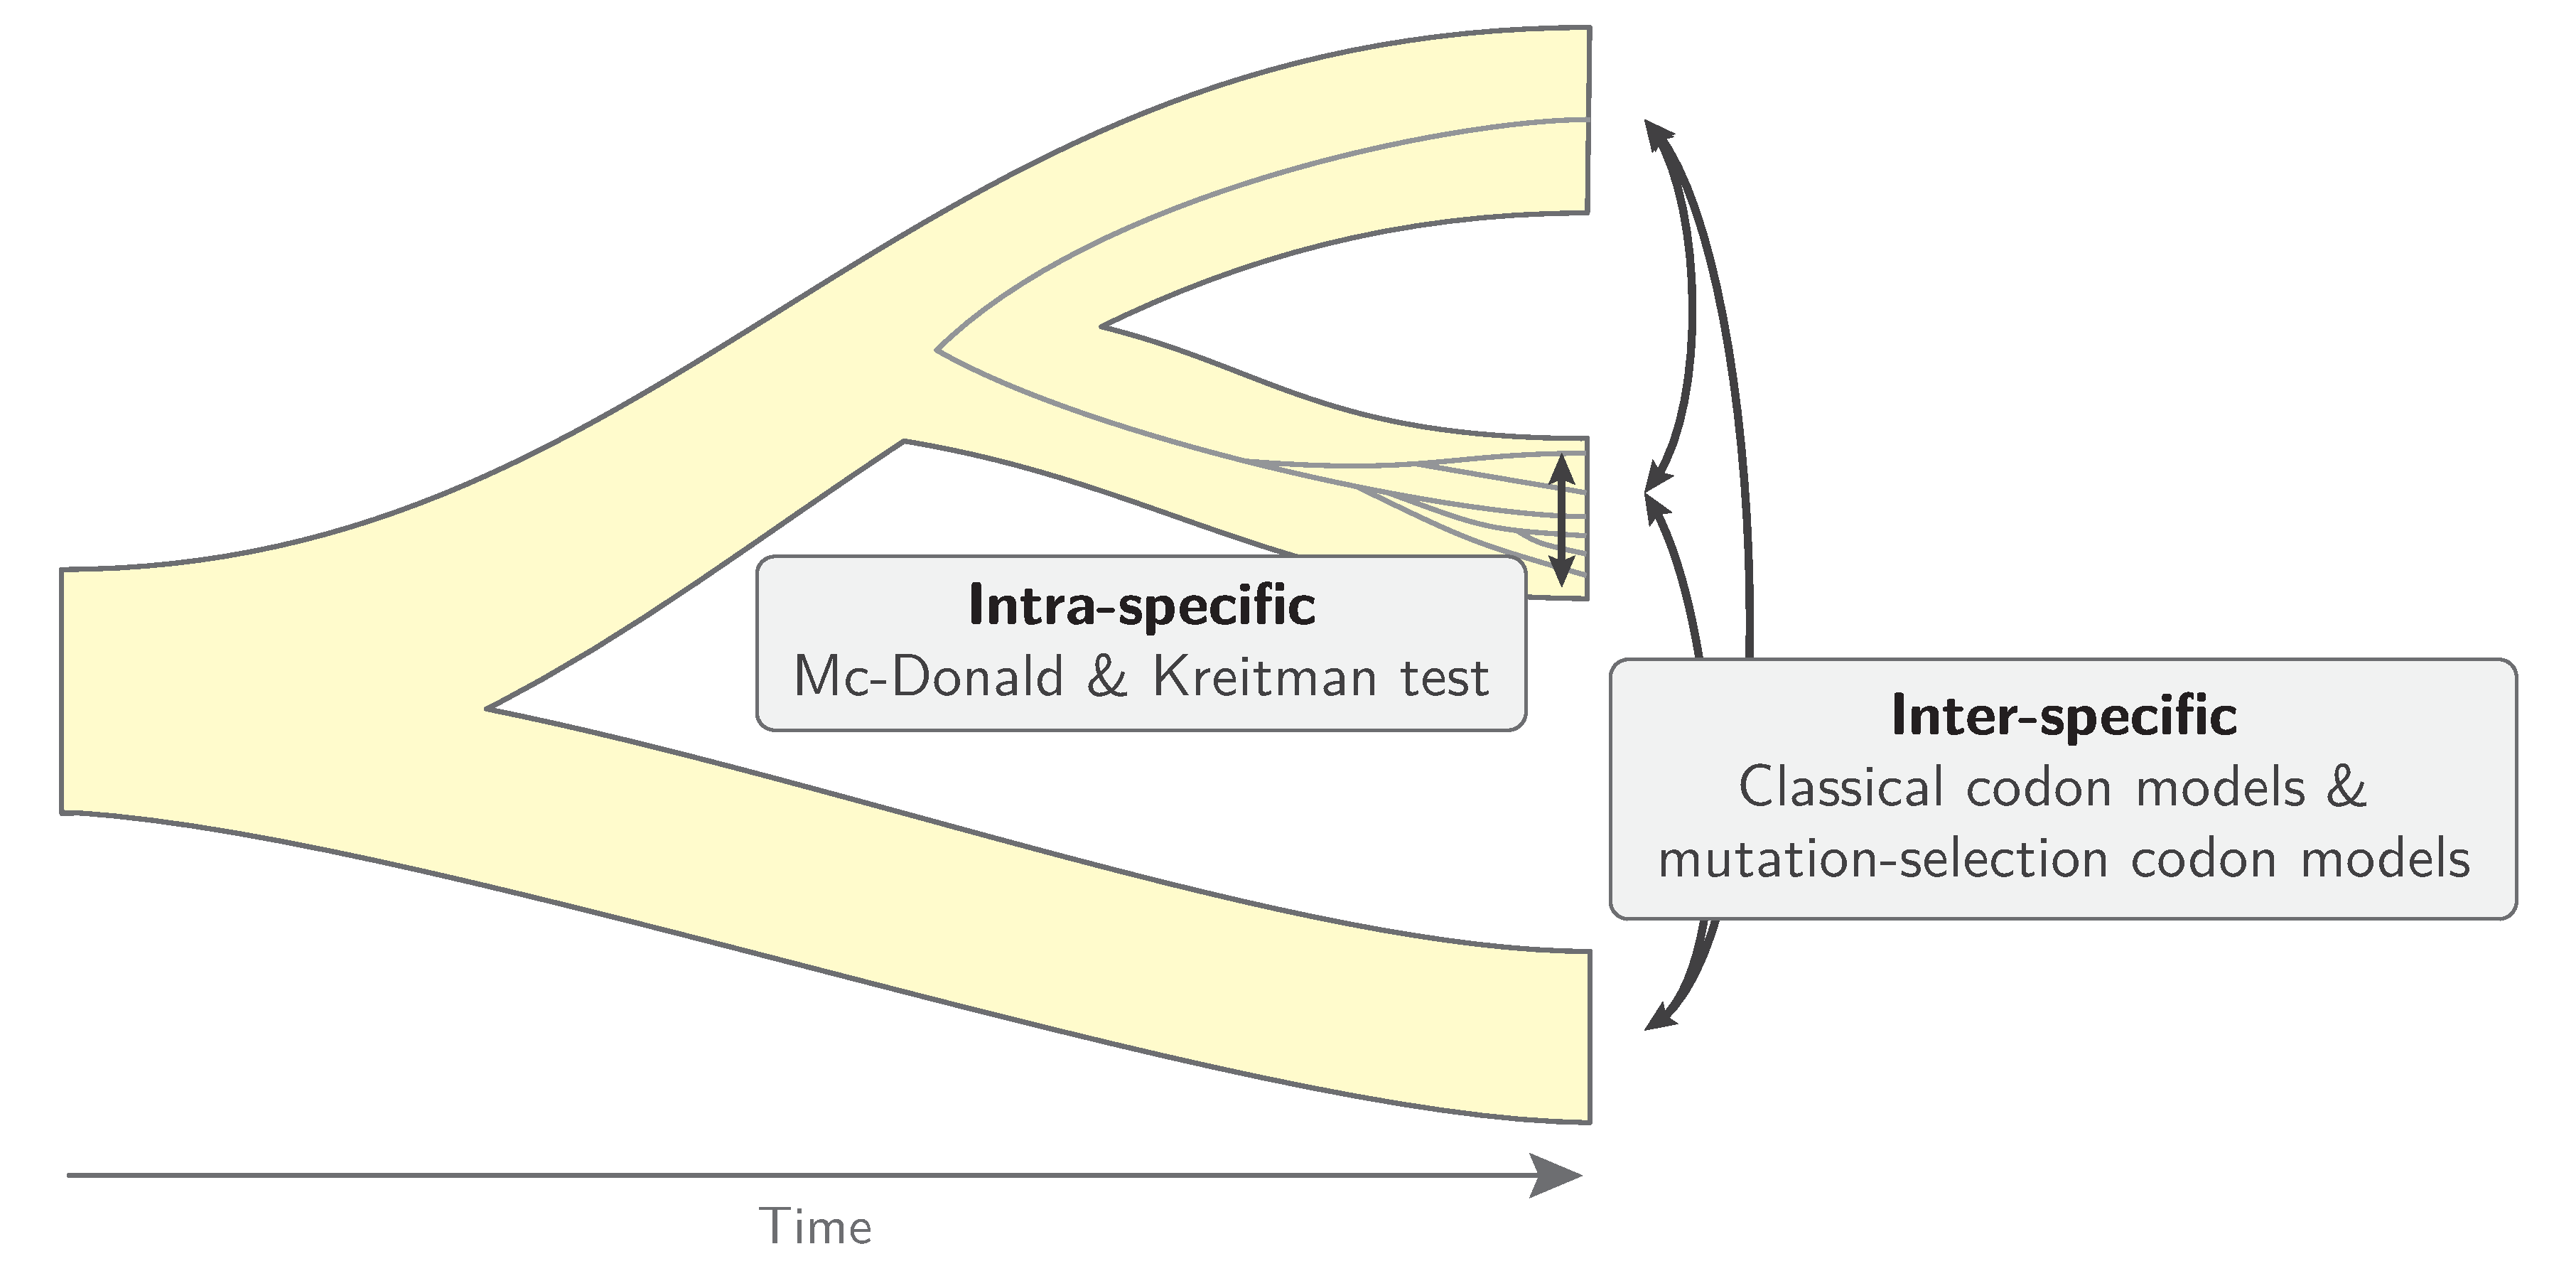
\includegraphics[width=\textwidth] {figures/inter-intra}
	\caption{Detecting adaptive evolution in coding sequences from inter- and intra-specific data}
\end{figure}

\subsection{Adaptive \gls{substitution} rate}
The population and phylogeny-based method work over very different time scales.
For that reason, they might be capturing different signals: isolated events of adaptation along a particular lineage for population-based method, versus long-term evolutionary Red-Queen for phylogeny based methods. On the other hand, the two signals might be correlated. This represent a unique opportunity to confound these two types of approaches on non-overlapping data frames. Accordingly, the goal of this study is to set-up a pipeline for gathering divergence and polymorphism data for coding genes across species. As a proof of concept, I analyzed 1,355 protein-coding sequences (CDS) orthologs in mammals, and conducted two separate analysis on these CDS. First, alignments in placentals (except \textit{Homo sapiens} and \textit{Pan troglodytes}) were used to run classical site-models and mutation-selection models. The method estimated the rate of adaptation in each CDS, and extracted CDS with a rate of adaptation significantly high. Secondly, the population-based method was conducted using polymorphism available in \textit{Homo sapiens} and divergence to \textit{Pan troglodytes}. The pipeline then testes if the group of sequences detected with a high rate of adaption in the phylogeny-based method also display a high rate of adaptation in the population-based method.

Finally, I investigated whether the phylogeny-based and the population-based methods give congruent results in terms of detection of adaptive evolution. 
To do so, $\omega_A^{MK}$ was computed on the concatenate of the $27$ candidates CDS inferred, by the phylogeny-based method, to have a high rate of adaptation. The result was compared to the empirical distribution of $\omega_A^{MK}$ over random sets of $27$ CDS.
The average rate of adaptation over the $27$ candidates, such as estimated by Mc-Donald and Kreitman (see methods), is higher than the average rate of adaptation over random samples. However, the deviation is not significant ($p_{\mathrm{value}}=0.119$).\\

Similarly, using the site-frequency spectra of SNPs, $\omega_A^{DFEM}$ was computed in the same set of candidates by concatenating the $27$ site-frequency-spectrum. And compared it to the empirical null distribution of $\omega_A^{DFEM}$ over random sets of $27$ CDS.
The average rate of adaptation over the $27$ candidates, such as estimated using the GammaExpo model (see methods), is higher than the average rate of adaptation over random samples. In this case, the deviation is marginally significant ($p_{\mathrm{value}}=0.036$), 
meaning that modeling change in population size and the distribution of fitness effects of mutations leads to more congruence between phylogeny and population-based methods, suggesting that the two methods are at least partially congruent in their detection of adaptation.

\subsection{Confronting inter and intra specific inference}

This study is the first medium-scale application of the phylogenetic mutation-selection method for detecting adaptation. The approach required some changes compared to the original method. More specifically, a two-step procedure was derived and deemed more reliable than the one-step approach of \citet{Lartillot2013}. This approach seems to give sensible results. Its application on mammalian CDS suggests that most proteins are under \textit{nearly-neutral} regime and a few candidate proteins are under strong adaptation. The protein under adaptation also showed significant increase in ontology terms related to immune processes. In practice, there could be some background adaption in proteins categorized here as being in a \textit{nearly-neutral} regime, which might not have been detected due to lack of power of the statistical test. Further work is also needed to compare with classical \gls{codon} models. Here, $27$ CDS were detected out of $1,355$. In \citet{kosiol_patterns_2008}, $400$ CDS were detected out of $16,529$ using \gls{codon} site-model, suggesting that the mutation-selection model has somewhat a lower, although comparable, sensitivity compared to site-model. Ultimately, I should first scale-up the analysis to the whole dataset of $11,256$ CDS, instead of the $1,355$ CDS used because of time and computation constrains. Indeed, phylogeny-based method is computationally intensive, and requires a well resolved species tree, hence the limitation to mammals in this study. Moreover it crucially depends on the quality of the alignments, as was observed in preliminary study, and paralogs identified as orthologs or alignment problems can easily falsify the results.\\

A second objective of this work was to confront phylogeny-based and population-based methods. One main novelty of mutation-selection model, compared to classical \gls{codon} models, is to provide an estimate of $\omega_A$, thus directly comparable with population-based methods. Ideally, one would like to make a quantitative comparison of $\omega_A$ and $\omega_A^{MK}$, across sequence or groups of sequences. However, the method lacked of power for two reasons. Firstly, the method did not detected enough CDS under adaptation ($27$ CDS with $\omega_A > 0$). Secondly the population-based estimation was very noisy, also requires concatenating many sequences. Nevertheless, these preliminary results are encouraging. Practically, it is possible to apply this pipeline to other species than \textit{Homo sapiens}, where \gls{polymorphic} diversity is greater such as \textit{Mus} (using the same mammalian phylogeny) or \textit{Drosophila} (with another phylogeny). \\

The set of CDS detected to be under adaptation in phylogeny-based methods showed a marginally significant increase in the rate of adaption, such as inferred by population-based method. This relatively weak correlation might just reflect the limited number of CDS analyzed and the limited statistical power of the population-based method mentioned above. However, it is also possible that the two methods are inherently testing for different patterns of adaptation, meaning that recent episode of adaptation in the \textit{Hominini} lineages do not reflect the long-term patterns of adaptation. Especially since the purifying process is stronger on longer timescale, the frontier between \gls{neutral} and mildly deleterious mutation is blurred on short timescale \citep{ho_time_2005}. \\

Altogether, this preliminary study suggest that the integration between population and phylogeny-based methods raises theoretical and practical issues. I suggest that further investigating these methodological integration will provide biological understanding of the evolutionary constrain of protein-coding sequences. \\


\section{Epistasis in molecular evolution}

\subsection{Definition of epistasis}

Yet another classification of epistasis, which is helpful in the context of protein evolution,
is specific epistasis and non-specific epistasis (56) (Figure 1). Specific epistasis is structural in origin and results from direct physical interaction of spatially close residues in a protein’s 3D structure. Mutations occurring at spatially proximate sites will have non-additive contributions to the biophysical properties of proteins such as stability, activity, dynamics, or binding with partner proteins (57). Specific epistasis may also arise through long-range allosteric effects of mutations that are spatially far apart as in the case of O2 affinity in mammalian and avian Hemoglobin(40; 34). If the biophysical properties determine organismal fitness, as recently shown in examples of viral and bacterial evolution (28; 8), the non-additivity at the level of proteins translates to non-additivity at the level of fitness. As a consequence, the rate and patterns of \gls{substitution} in one site may be correlated with that of another spatially close site (58; 39; 36; 46; 19).

On the other hand, non-specific epistasis arises from the non-linear dependence of
cellular/organismal fitness to biophysical properties such as folding stability (Figure 1). Even if biophysical properties are additive, the non-linear mapping of the biophysical property to fitness introduces non-linear interactions among mutations at the fitness level. Since Darwinian selection acts at the level of organismal fitness, non-specific epistasis could also affect the rate of evolution. The simplest mapping between fitness and protein properties exhibits a singlepeak, such as shown in Figure 1 for folding stability. This plateau-like fitness landscape has also been shown for the relationship between fitness and the intracellular abundance of a gene (5), between fitness and enzyme activity (26; 23; 48), and between fitness and folding stability[33]. In these simple landscapes, non-specific epistasis gives rise to the “law of diminishing returns”, i.e., the selective advantage of mutations decreases as the fitness of the organism increases, a well-known feature of many optimization processes and in adaptive trajectories in protein evolution (31; 14; 38).

\textbf{Estimating the contribution of folding stability to nonspecific epistasis in protein evolution }
The extent of nonadditive interaction among mutations or epistasis reflects the ruggedness of the fitness landscape, the mapping of genotype to reproductive fitness. In protein evolution, there is strong support for the importance and prevalence of epistasis but the quantitative and relative contribution of various factors to epistasis are poorly known. Here, we determine the contribution of selection for folding stability to epistasis in protein evolution. By combining theoretical estimates of the rates of molecular evolution and the nonlinear mapping between protein folding thermodynamics and fitness, we show that the simple selection for folding stability imposes at least ~30\% to ~40\% epistasis in long-term protein evolution. Estimating the contribution of governing factors in molecular evolution such as protein folding stability to epistasis will provide a better understanding of epistasis that could improve methods in molecular evolution.
 \citet{Dasmeh2018}


Building upon this computational convenience, complex models that allow for lineage-specific rate shifts have been developed to phenomenologically (nonmechanistically) treat signal that may originate from site-interdependence.
Gaucher EA, Gu X, Miyamoto MM, Benner SA (2002) Predicting functional divergence in protein evolution by site-specific rate shifts. Trends Biochem Sci 27: 315–321.
Whelan S, Blackburne BP, Spencer M (2011) Phylogenetic \gls{substitution} models for detecting heterotachy during plastid evolution. Mol Biol Evol 28:449–458.


Models of protein evolution that incorporate pro-
tein structure have been shown to fit data better than the corresponding models that ignore protein structure. However, an even better fit to the data could be achieved with state-of-the-art site-independent \gls{codon} models.42 Despite their having parameters with biologically meaningful explanations, the lackluster statistical fit of dependent site models is clearly disappointing.
41. Rodrigue N, Philippe H, Lartillot N (2006) Assessing site-interdependent phylogenetic models of sequence evolution. Mol Biol Evol 23:1762–1775.
42. Rodrigue N, Kleinman CL, Philippe H, Lartillot N (2009) Computational methods for evaluating phylogenetic models of coding sequence evolution with dependence between \glspl{codon}. Mol Biol Evol 26: 1663–1676

\subsection{Epistasis and rate of evolution}

Previous studies have argued that models of molecular evolution should consider the importance epistasis for its role in speciation, in modulating the rate of adaptation, and many other factors \citep{Goldstein2017, Miller2018}.
We argue that epistasis also has an important role in the response of $\omega$ to changes in $\Ne$, both in terms of susceptibility and dynamic of the response.
Fundamentally, we argue that any model modeling fitness at the site level (without epistasis) implies a slow dynamic and a strong susceptibility, and adding epistasis to the model imply a faster dynamic and a weaker susceptibility.
Intuitively, this effect originates in the fact that each site is to adapt independently to changes in $\Ne$ leading to overall a slow response (substitutions must affect all sites), and a strong susceptibility since each site will change its position in the fitness landscape.
Taking into account epistasis, the burden of adapting to changes in $\Ne$ is shared by more sites, such that all of them don't have to adapt. 
From a modeling and inference perspective, accounting for epistasis is challenging both in terms of parametrization and computational complexity \citep{Rodrigue2005, Manhart2014}. 


\section{Reproducible science}
I argue that analytical models, computational simulations and inference models are complementary, but more importantly they are necessary to each others. 
Theoretical modeling allow to understand the principles, simulations allow to verify the soundness.
Inference allow to extract and test the theoretical results using empirical data.
Simulations have a dual role, testing the robustness of both inference procedures and theoretical results, outside of their comfort zone and assumptions.
However, this assume we are confident enough to write reproducible computations, as such the next section is dedicated to my personal experience and take away.

\subsection{Reproducible computations}
First, I stand firmly on the ground that data, codes and scripts should be rendered open-access of any published and peer reviewed paper.
Practically, the availability of the data and source code should simply be enforced upon submission to journal, which is currently not the case for all journals, even in bio-informatics and genomics fields.
It is true that such enforcement bears the consequence to weight more burden on scientists upon publishing.
However, it avoids the bloating of technical debt, or research debt where we build on the ground of a dangerous and possibly shaky basement.
It encourages peer collaboration, both helping the team or person whom made the code available, and the community as a whole.
A straightforward way is to provide a \textit{git} versioned repository, with the advantage that collaboration is facilitated trough web hosted repository such as GitLab (hosted by institutions) or GitHub (hosted by Microsoft).

Nonetheless, code availability is a necessary condition, but not the sole requirement of reproducible research.
Specific instructions to reproduce the results should also be made available, where many tools are available to this aim \citep{Wilson2014,Darriba2018}.
The first step necessary to reproduce a code is to have the required environment, meaning the necessary libraries and dependencies of the code and scripts.
For script and code written in Python, the package manager anaconda (or conda) provides a straightforward environment to configure the necessary libraries with their versions. 
More complex environment requiring code compilation or system-level packages can leverage containerization technology such as Docker or Singularity for example, but any other containers implementing system-level virtualization is very helpful to provide the necessary libraries.
Once the environment is specified, the documentation can be made available as a README with the necessary instructions.
More generally, notebooks such as \textbf{Jupyter Notebook}, \textbf{RMarkdown} or \textbf{org-mode} to name a few also provide an environment knitting together code and instructions, allowing to follow step-by-step experiments, analysis and results, in a similar fashion as laboratory notebook which are strictly required in wet labs.
It is important to note that notebooks can run code from a variety of languages (C++, Haskell, Java, Julia, Python, Wolfram Language, Matlab, Ruby, ...).
These tools are emerging in the community, as well as Workflow management system (Nexflow, Snakemake, etc) allowing to create reproducible and scalable data analyses running on computing clusters.

Using this range of tools helps other scientists which might want to understand, test or build upon published works. 
Moreover, they are also very helpful for the person or team implementing them since a more rigorous and reproducible environment allows to more easily track down bugs and test programs under different conditions or dataset\footnote{Notebooks are very useful to present work and data analysis, but should not be used during development since they often offers poor integration with debugger and code inspection tools, enforce awkward software design patterns, and often result in bloated versioned repository.}. 
During the development period, continuous integration pipelines are valuable to increase the reliability of code generation, which should be used whether working alone or inside team, but is of course more critical for collaborative code where one cannot control all the code written.
Collaborative coding practices such as peer-coding sessions is really useful to implement critical code at the core of the program under development.
I argue that the efficiency peer-coding sessions is provided by dividing the tasks into a group focused in the detailed implementation while the others a free to focus on edge cases and the overall implication of different implementations. 
Moreover, peer-coding sessions provides a convenient and structured place for learning good practices, for expanding its technical knowledge while pruning bad habits.
An other remarkable practice is to write two independent version of the program, using if possible different algorithm and languages but with the same functionality, but most importantly by a different person.
Then testing the program against each others on the same conditions and dataset should result in the same outcome\footnote{An extreme version is adversarial coding (or chaos engineering), where the goal is to find conditions on which the adversary program fails.}.
Such model of reproducible computing experiment and analysis is laborious and demanding, but I argue this is the definition of reproducibility we collectively should aim for, namely where one can independently reproduce the same experiment, and if reproducibility fails one can run the code with different conditions to pinpoint the failing code (which might actually be in both versions).
Personally, having practiced this method I strongly believe it pervasively reduces our research debt that we might inadvertently burden other with whenever not realizing the program is bugged, and ultimately save us time on debugging and research conduction.
Finally, explaining to others our choices of algorithms, implementation and data structure requires us to express intelligibly our mental ideas and therefor better understand them, while gaining from others insight and algorithmic expertise.

\subsection{Bayesian statistics}
Knowingly that maximum \gls{likelihood} and Bayesian statistics are often opposed to each others and sometimes fiercely defended by their tenant, using one of them implicitly put someone in the position to argument their choice. 
Bayesian statistics seems personally a more comfortable inference framework than maximum \gls{likelihood} for several reasons. 
Firstly, you technically are not required to devise procedure necessary to evades local optimums.
Second and most importantly, Bayesian statistics output not a single statistic but a confidence interval, meaning how much certainty is available given the data.
Posterior and \gls{prior} can be thus presented next to each others and differences between the two is due to signal extracted from the data.
A corollary is that over parametrization is not such a drastic issue as in maximum \gls{likelihood} inference, since in a case where there is only limited extractable signal from the data this will reflect in the confidence interval.
In the worst possible case of over parametrization, namely that of confounded parameters and the model is exactly the same for different set of parameters, the confidence interval will expand but confounded parameters can be identified afterward through parameters correlation in their joint \gls{posterior} distribution.
The subjective arbitrary introduced by lasso and penalized-likelihood is replaced by statistical \gls{prior} distribution.
However, over-parameterized models is still a misappropriate use of computing resource, which results in a greater environmental cost.

Relationship between \gls{prior} and \gls{posterior} allows for a simple, thought extensive method to test for the repeatability and soundness of the inference code with regard to simulations.

For a given parameter  can be draw from the \gls{prior} distribution, simulations run with this specific parameters, and for each simulation an inference result in an average \gls{posterior} estimate.






